%%%%%%%%%%%%%%%%%%%%%%%%%%%%%%%%%%%%%%%%%
% a0poster Landscape Poster
% LaTeX Template
% Version 1.0 (22/06/13)
%
% The a0poster class was created by:
% Gerlinde Kettl and Matthias Weiser (tex@kettl.de)
% 
% This template has been downloaded from:
% http://www.LaTeXTemplates.com
%
% License:
% CC BY-NC-SA 3.0 (http://creativecommons.org/licenses/by-nc-sa/3.0/)
%
%%%%%%%%%%%%%%%%%%%%%%%%%%%%%%%%%%%%%%%%%

%----------------------------------------------------------------------------------------
%	PACKAGES AND OTHER DOCUMENT CONFIGURATIONS
%----------------------------------------------------------------------------------------

\documentclass[a0,landscape]{a0poster}

\usepackage{multicol} % This is so we can have multiple columns of text side-by-side
\columnsep=100pt % This is the amount of white space between the columns in the poster
\columnseprule=3pt % This is the thickness of the black line between the columns in the poster

\usepackage[svgnames]{xcolor} % Specify colors by their 'svgnames', for a full list of all colors available see here: http://www.latextemplates.com/svgnames-colors

\usepackage{times} % Use the times font
%\usepackage{palatino} % Uncomment to use the Palatino font

\usepackage{graphicx} % Required for including images
\graphicspath{{figures/}} % Location of the graphics files
\usepackage{booktabs} % Top and bottom rules for table
\usepackage[font=small,labelfont=bf]{caption} % Required for specifying captions to tables and figures
\usepackage{amsfonts, amsmath, amsthm, amssymb} % For math fonts, symbols and environments
\usepackage{wrapfig} % Allows wrapping text around tables and figures
\usepackage{enumitem}
\usepackage{listings}% http://ctan.org/pkg/listings
\usepackage{algorithm}
\usepackage{algpseudocode}
\usepackage{mathtools}
\lstset{
  basicstyle=\ttfamily,
  mathescape
}
\usepackage{pgf,tikz}
\usepackage{pgfplots}
\pgfplotsset{compat=newest}

\DeclareMathOperator{\rank}{rank}
\DeclareMathOperator{\spann}{span}
\newcommand\SPAN[1]{\ensuremath\spann(#1)}

\newtheorem{thm}{Theorem}
\newtheorem{lemma}{Lemma}
%\newtheorem{proposition}{Proposition}
\newtheorem{coro}{Corollary}
%\newtheorem{definition}{Definition}
\newtheorem{remark}{Remark}

\begin{document}

%----------------------------------------------------------------------------------------
%	POSTER HEADER 
%----------------------------------------------------------------------------------------

% The header is divided into three boxes:
% The first is 55% wide and houses the title, subtitle, names and university/organization
% The second is 25% wide and houses contact information
% The third is 19% wide and houses a logo for your university/organization or a photo of you
% The widths of these boxes can be easily edited to accommodate your content as you see fit

\begin{minipage}[b]{0.58\linewidth}
  \veryHuge \color{NavyBlue} \textbf{Automatic Differentiation} \color{Black}\\ % Title
  \Huge\textit{Inside the Black Box at the Heart of Machine Learning}\\[1cm] % Subtitle
  \huge \textbf{Damion A.~Miller}\\ % Author(s)
  \huge Michigan Tech\\ % University/organization
\end{minipage}
%
\begin{minipage}[b]{0.22\linewidth}
  \Large \textbf{Contact Information:}\\
  Damion A.~Miller\\
  Michigan Technological University\\
  Department of Mathematical Sciences \\
  Houghton, MI\\\\
  Email: \texttt{damionm@mtu.edu}\\ % Email address
\end{minipage}
%
\begin{minipage}[b]{0.19\linewidth}
  
\includegraphics[width=20cm]{figures/logo.png} % Logo or a photo of you, adjust its dimensions here\\
  \vspace*{2in}
\end{minipage}

\vspace{1cm} % A bit of extra whitespace between the header and poster content

%----------------------------------------------------------------------------------------

\begin{multicols}{4} % This is how many columns your poster will be broken into, a poster with many figures may benefit from less columns whereas a text-heavy poster benefits from more

%----------------------------------------------------------------------------------------
%	ABSTRACT
%----------------------------------------------------------------------------------------

\begin{abstract}
    Automaic differentiation (AD) if a method for accurately and efficiently
    computing derivativatives of functions. I explore two different methods
    of AD both having different pros and cons, as well as different combinations
    of these methods all with unique outcomes. Using these results we are able to
    apply them to many applications such as machine learning or solving differential
    equations.
\end{abstract}

%----------------------------------------------------------------------------------------

\section*{Motivation}
\begin{itemize}[noitemsep]
\item Derivatives are present in almost all areas of engineering.
\item Especially relevant in machine learning where the gradient (a derivative
    in the direction of steepes ascent) must be calulated large numbers of times
    over functions with large input vectors.
\item Find efficient algorithms for solving different problems involving derivatives
    using purposefully choosen combinations of AD.
\end{itemize}
    \vspace{-1cm}
\section*{Computational Graph}
    Let $f:\mathbb{R}^n\rightarrow\mathbb{R}$ and $\vec{x}=(x_1,x_2,\dots,x_n)^T\in\mathbb{R}^n$

    Then one of four cases (Binary, Unary, Trivial, Constant):
\begin{align*}
    1.\ f(\vec{x})&=g(\vec{x})\odot h(\vec{x}) &&\odot\in\{+,-,*,/,\dots\} \\
    2.\ f(\vec{x})&=g(h(\vec{x})) &&g(x)\in\{\cos{(x)},\sin{(x)},\exp{(x)},\log{(x)},\dots\} \\
    3.\ f(\vec{x})&=x_i &&1\leq i\leq n \\
    4.\ f(\vec{x})&=\alpha &&\alpha\in\mathbb{R}
\end{align*}

Now recurse on $h(\vec{x})$ and $g(\vec{x})$ in case 1 until case 3 or 4 returned.
At this point we have what is known as a computational graph of $f(\vec{x})$.

\begin{center}
    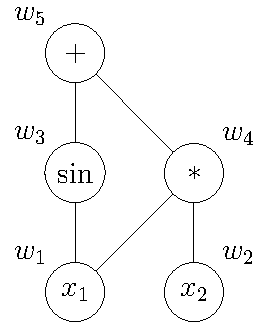
\includegraphics[width=100mm]{figures/comp_graph.pdf}
    \captionof{figure}{Computational graph of $f(x_2,x_2)=x_1*x_2+\sin{(x_1)}$}
\end{center}

    \section*{Forward Mode}
\begin{thm}
    Let $l(\vec{x}):\mathbb{R}^n\rightarrow\mathbb{R}$ be the function $l(\vec{x})=x_i$ where $\vec{x}^T=(x_1,x_2,\dots,x_n)$ and $1\leq i\leq n$.
    Let $\vec{z}\in\mathbb{R}^n$ be a unit vector. 
    Then $\frac{\partial}{\partial\vec{z}}l(\vec{x})=z_i$.
    \begin{proof}
        $$\frac{\partial}{\partial\vec{z}}l(\vec{x})=\lim_{h\rightarrow0}\frac{l(\vec{x} + h\vec{z}) - l(\vec{x})}{h}=\lim_{h\rightarrow0}\frac{x_i + hz_i - x_i}{h}=z_i.$$
    \end{proof}
\end{thm}

Using this information, functions and their derivatives with respect to a direction,
we can easily obtain the composition function and its derivative with repect to that direction.

Case 1: Binary (product rule, quotient rule, etc.) 

    Given $(g(\vec{x}),\frac{\partial g}{\partial\vec{z}}),(h(\vec{x}),\frac{\partial h}{\partial\vec{z}})$,and $f(\vec{x})=g(\vec{x})\odot h(\vec{x})$
    \begin{equation}
        \frac{\partial f}{\partial\vec{z}}=
            \begin{cases}
                \frac{\partial g}{\partial\vec{z}} + \frac{\partial h}{\partial\vec{z}} & \text{if } \odot = +\\
                \frac{\partial g}{\partial\vec{z}} - \frac{\partial h}{\partial\vec{z}} & \text{if } \odot = -\\
                g(\vec{x})\frac{\partial h}{\partial\vec{z}} + h(\vec{x})\frac{\partial g}{\partial\vec{z}} & \text{if } \odot = *\\
                \frac{h(\vec{x})\frac{\partial g}{\partial\vec{z}} - g(\vec{x})\frac{\partial h}{\partial\vec{z}}}{(h(\vec{x}))^2} & \text{if } \odot = /\\
                \dots
            \end{cases}
    \end{equation}

Case 2: Unary (chain rule)

    Given $(h(\vec{x}),\frac{\partial h}{\partial\vec{z}})$ and $f(\vec{x})=g(h(\vec{x}))$
    \begin{equation}
        \frac{\partial f}{\partial\vec{z}}=\frac{\partial}{\partial\vec{z}}g(h(\vec{x}))=\underbracket{\frac{dg}{dh}}_{\text{trival}}*\underbracket{\frac{\partial h}{\partial\vec{z}}}_{\text{given}}
    \end{equation}
    \begin{equation}
        \frac{dg}{dh}=
            \begin{cases}
                \cos{(h(\vec{x}))} & \text{if } g(x) = \sin{(x)}\\
                -\sin{(h(\vec{x}))} & \text{if } g(x) = \cos{(x)}\\
                \exp{(h(\vec{x}))} & \text{if } g(x) = \exp{(x)}\\
                \frac{1}{h(\vec{x})} & \text{if } g(x) = \log{(x)}\\
                \dots
            \end{cases}
    \end{equation}

Using the above relations we are able to build up from trivial functions and their corresponding
derivatives until we obtain our original function and its derivative in the desired direction.
\vspace{-1cm}
\subsection*{Implementation}
\vspace{-1cm}
\begin{center}
    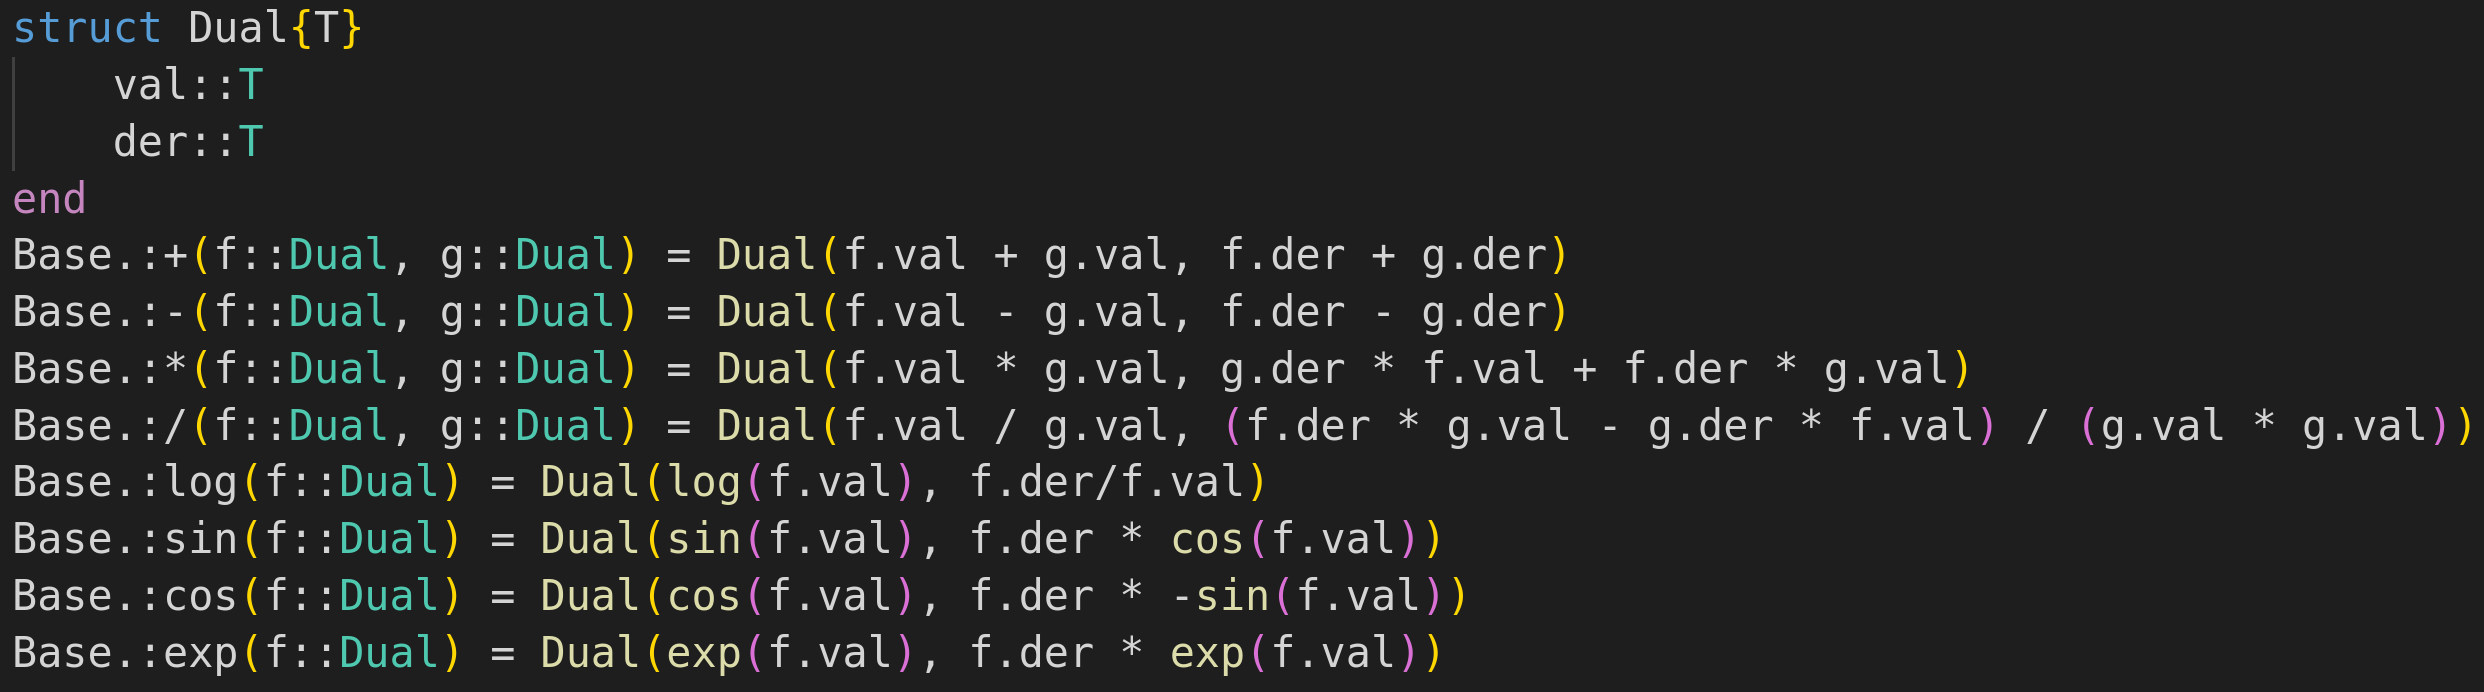
\includegraphics[width=250mm]{figures/forward_mode.png}
    \captionof{figure}{Simple forward mode implementation in Julia using Dual numbers and operator overloading.}
\end{center}
\vspace{-1cm}
\subsection*{Algorithm}
    \textbf{Input:} \\ 
    $f(\vec{x}):\mathbb{R}^n\rightarrow\mathbb{R}$ \quad \textit{function} \\
    $\vec{x}\in\mathbb{R}^n$ \quad \textit{input point} \\
    $\vec{z}\in\mathbb{R}^n$ \quad \textit{direction} \\
    \textbf{Output:} $(f(\vec{x}),\frac{\partial}{\partial\vec{z}}f(\vec{x}))$ \\
    $D\leftarrow$ Initialized vector of $n$ Dual numbers \\
    \textbf{for } $i\leftarrow1$\textbf{ to } $n$ \\
    $\text{    } D[i]\leftarrow Dual(x_i, z_i)$ \\
    \textbf{return} $f(D)$ \\

We simply have to do the upfront work of mapping the original input vector to 
a vector with dual number components, each with a derivative value equal to the
corresponding component from the direction vector (Threorem 1). Then, once the function
is called on the dual number vector the evaluation of the function will be equivalent
to recursively breaking down the function until case 3 or 4 is obtained, from which 
the function and its derivative can be built up from, which is all handled via operator
overloading.

\section*{Reverse Mode}

\subsection*{Adjoint}
The adjoint is a key idea essential to reverse mode. 
The adjoint of a node in our compuational graph is simply the deriviative of the
overall function with respect to that nodes function.

\subsubsection*{Key Observations}
Let $P$ be the set of parents of the node whos function is equal to $x_i$, then
$$\frac{\partial f}{\partial x_i}=\sum_{w\in P}{\frac{\partial f}{\partial w}\frac{\partial w}{\partial x_i}}$$

The final node in our compuation graph has an adjoint of 1.

By starting at the top of our computational graph we can traverse the graph
from the top down, updating the adjoint values as we go, to compute the adjoint 
of each input node.

This can be done in time proportional to the original function and obtains the derivatives
in $n$ elementary directions which is the gradient of the function.

\subsection*{Implementation}
For implementation we use a tape, or array of nodes which represents our computation graph.
If one were to traverse this tape it would be equivalent to evaluating the function.
Obviously we don't wish to evaluate the function we want to calculate the adjoint of 
all the nodes within the tape. To do this we set the final nodes adjoint to 1.
Now for each node we need to visit its children (at most 2) and update their adjoint values.
To do this we need the childrens values, and the adjoint of their parent. Then we 
will simply add the product of the adjoint and the derivative of the parent with repsect to
the child to the childs adjoint.

\subsubsection*{Node}

\subsubsection*{Operator Overloading}
Similar to forward mode, we will use operator overloading to build our tape, that
is whenever an operation is called on two nodes, we wish to add a new node
representing its composition function to the end of our tape.

\subsection*{Algorithm}
Initialize $n$ nodes with values corresponding to the input to be the first $n$ nodes in the tape. \\
Call the function on the vector that is the first $n$ elements of the tape. \\
Set the adjoint of the final vector to be 1. \\
Traverse the tape backwards updating the adjoint of the children that compose each node. \\
Return the adjoint of the first $n$ nodes in the tape. \\

\section*{Higher Order Derivatives}
Calculating an order $n$ derivivative simply involves performing forward and/or reverse mode
$n$ total times. This allows for the derivative(s) calculated in the previous pass to
have a derivative component themselves.

\subsection*{Forward Forward}
By far the simplest higher order derivative example would be second order derivatives using
two forward passes. This is done by having a Dual number with Dual numbers for the value and
derivative componenents. The process is very similar, just initialize a vector of
these double dual numbers, giving the value component a derivivative component 
pertaining to the second direction and the derivative component a value component pertaining
to the first direction. After calling the function on these double dual numbers double
dual number returned will have the second derivative with respect to both directions provided
in derivative component of the derivative component. This can be and has been implemented
for $n$ order derivatives.

\subsection*{Reverse Forward}
Reverse Forward involves constructing a tape of Nodes with Dual numbers for the
adjoint component. This allowed for us to calculate the gradient efficiently and
then take the derivivaive with respect to a preallocated direction of the entire
gradient, yielding $n$ second order derivatives in time proporitional to the 
evaluation of the function. 

\subsection*{Forward Reverse}
Forward Reverse involves using Dual numbers with Node components, to construct a 
tape that can evaluate both the function and its derivative in a specified direction.
Then by setting the adjoint of the derivative function to 1 and rewinding the tape
we obtain the gradient of the derivavtive in a given direction. This has many applications
to machine learning.
\end{multicols}
\end{document}
